\section{Results And Tests}
Tests of both the device driver and the game were carried out continuously as the development progressed. These tests were all simple test to verify correctness. These can be presented as simple unit tests. A summary of some of the tests can be seen below.

\subsection{Energy usage results}

\begin{figure}[H]
  \centering
  % Trim er [left bottom right top]
  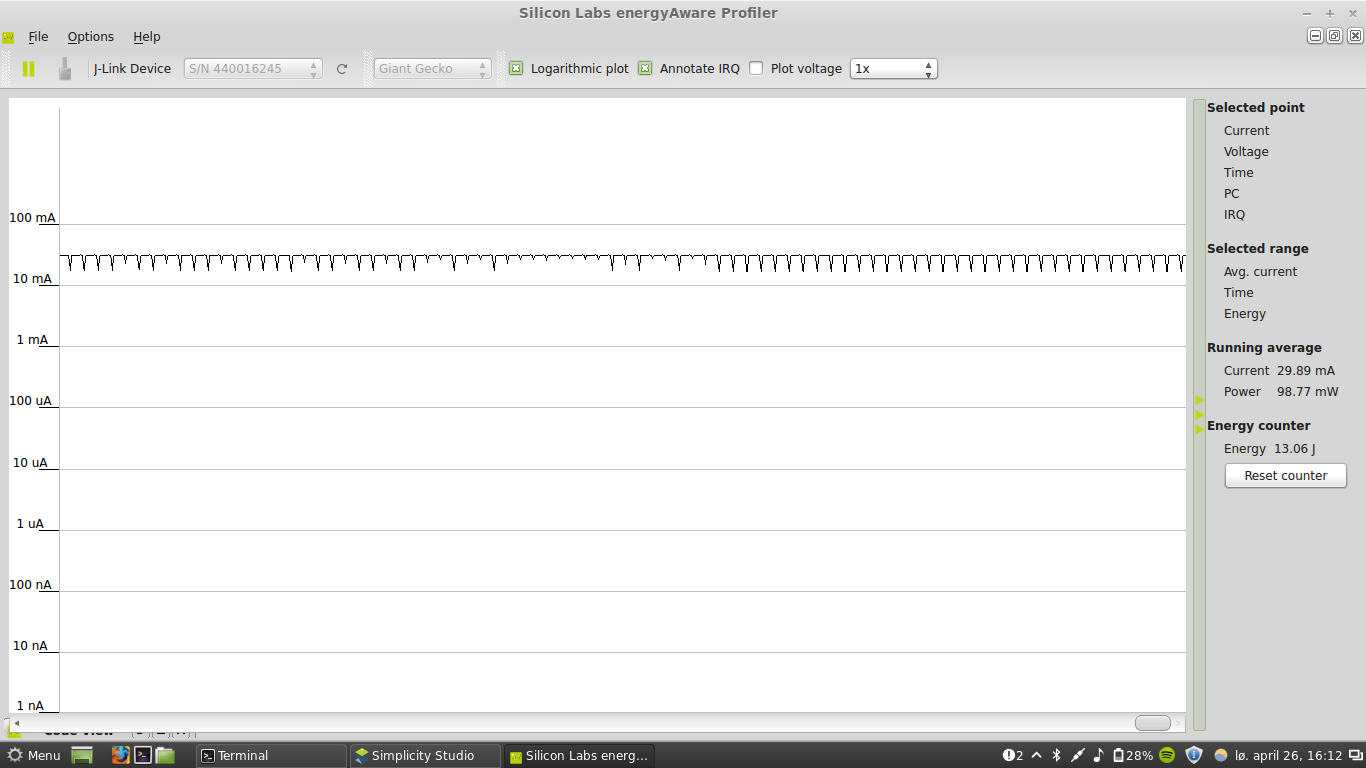
\includegraphics[clip, trim=0cm 0cm 0cm 0cm, width=12cm]{fig/runningIdle.png}
  \caption{Pong game running with tickless idle configuration}
\end{figure}

\begin{figure}[H]
  \centering
  % Trim er [left bottom right top]
  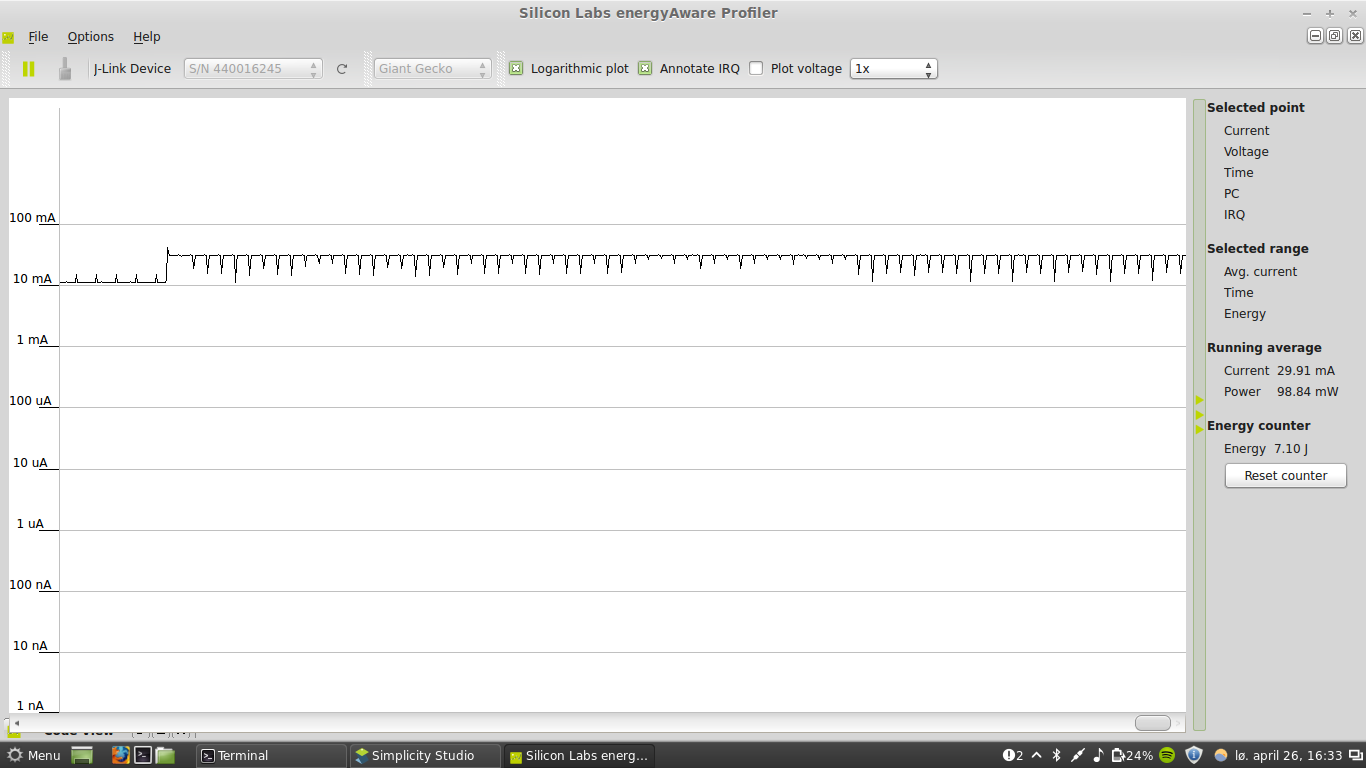
\includegraphics[clip, trim=0cm 0cm 0cm 0cm, width=12cm]{fig/running.png}
  \caption{Pong game running without tickless idle configuration}
\end{figure}

\begin{figure}[H]
  \centering
  % Trim er [left bottom right top]
  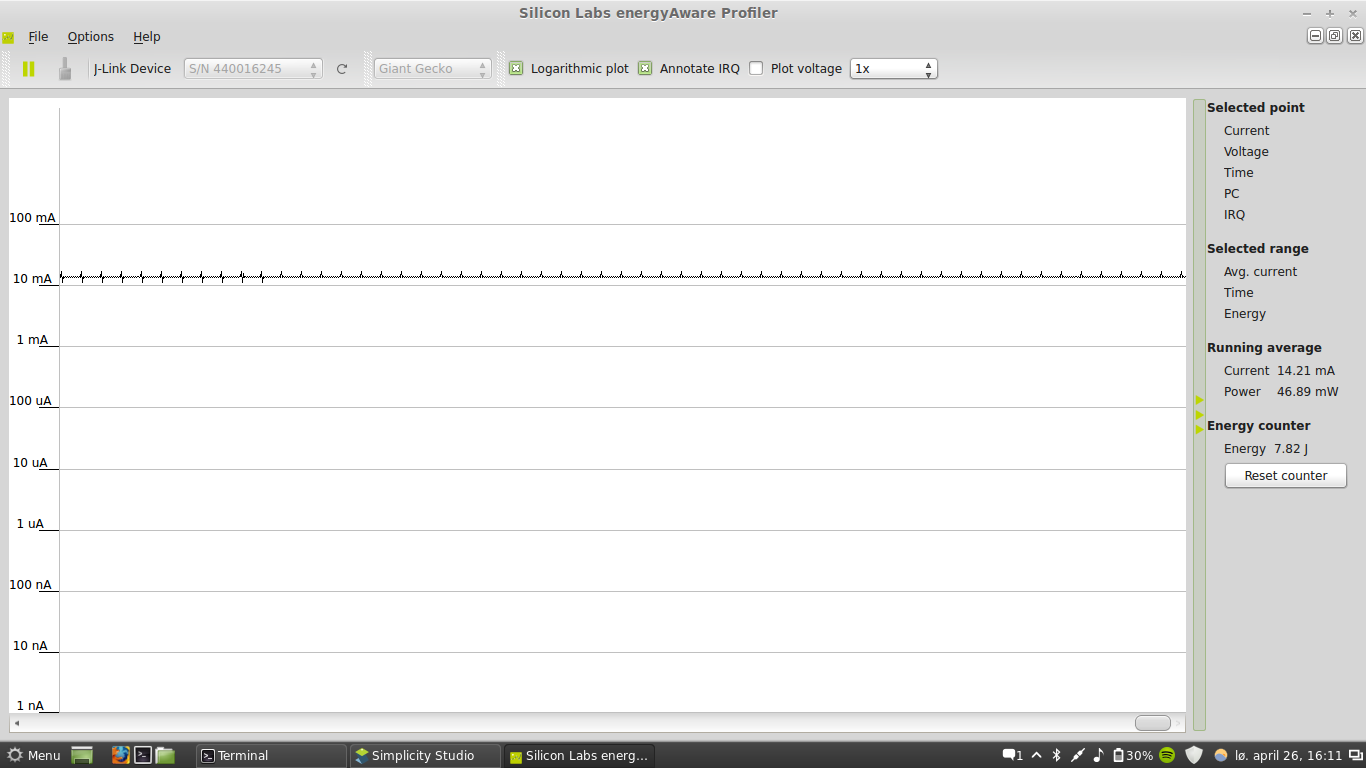
\includegraphics[clip, trim=0cm 0cm 0cm 0cm, width=12cm]{fig/victoryscreen-idle.png}
  \caption{Victory screen displayed with tickless idle configuration}
\end{figure}

\begin{figure}[H]
  \centering
  % Trim er [left bottom right top]
  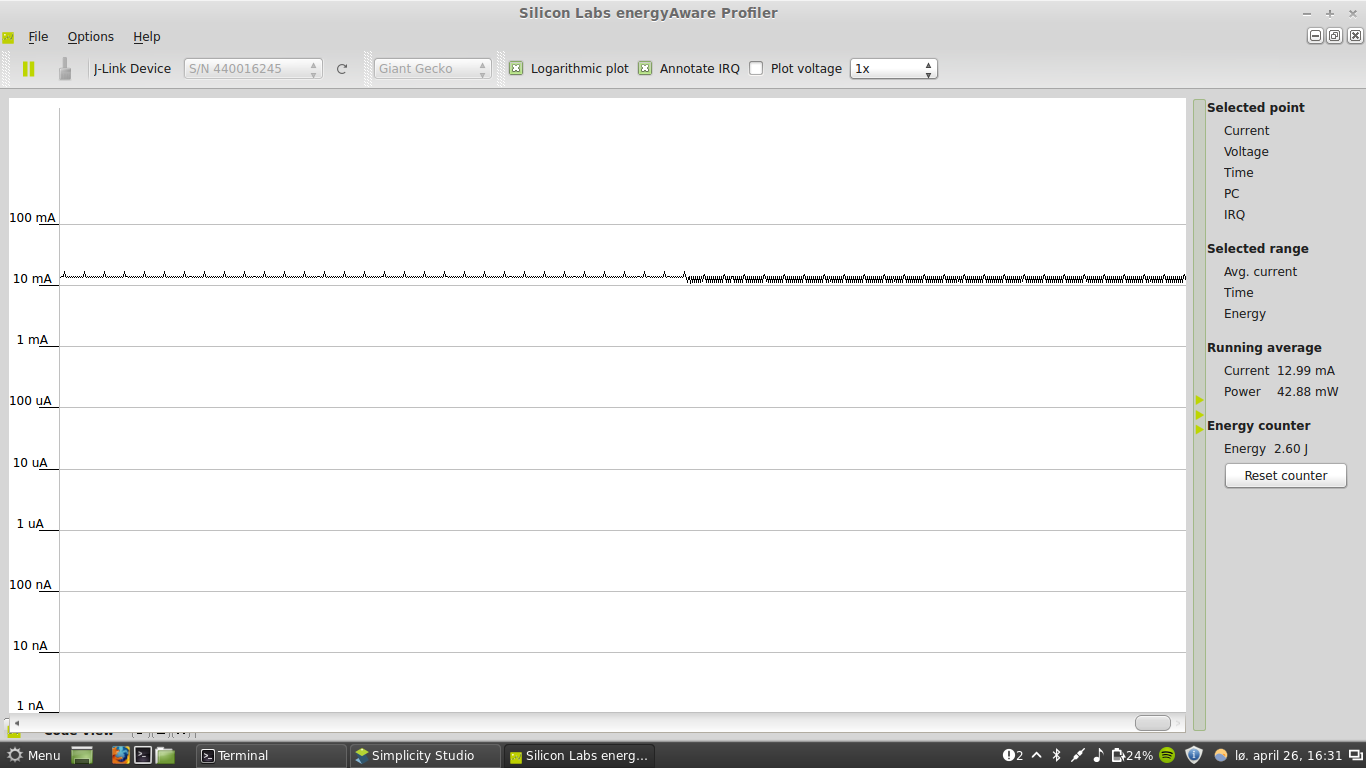
\includegraphics[clip, trim=0cm 0cm 0cm 0cm, width=12cm]{fig/Victory.png}
  \caption{Victory screen displayed with tickless idle configuration, with an average current of 12.99 mA}
\end{figure}




\subsection{Tests}

Following are test cases to see if the driver and the game behaves as expected

\subsubsection{Driver tests}

\emph{Input: } Load driver through the miniterm.py command line interface with the command "modprobe driver-gamepad"\\
\emph{Expected output: } Gamepad driver is successfully loaded, displaying message "Device added to the kernel sucessfully"\\
\emph{Actual output: } As expected\\

\emph{Input: } Unload driver through the miniterm.py command line interface with the command "rmmod driver-gamepad"\\
\emph{Expected output: } Gamepad driver is successfully unloaded, displaying message "Device added to the kernel sucessfully"\\
\emph{Actual output: } As expected\\

\emph{Input: } Load the driver through miniterm.py command line interface with the command "modprobe" driver-gamepad". Each button is pushed one by one.\\
\emph{Initial setup: } The interrupt handler is configured to print "Interrupt" for each interrupt.\\
\emph{Expected output: } The gamepad driver should be able to sense interrupt.\\
\emph{Actual output: } As expected. \\ 

\emph{Input: } Start the game through miniterm.py  \\
\emph{Initial setup: } The gamepad driver is loaded. Print message when FASYNC flag is set.\\
\emph{Expected output: } The device driver should detect that the FASYNC flag is set, E.g $fasync\_handler()$ is called.\\ 
\emph{Actual output: } As expected. \\






\subsubsection{Game tests}

The following unit tests are based on the gamepad driver having already been successfully added to the kernel, and takes a complete run-through of the game.

\emph{Input: } Start the game through miniterm.py\\
\emph{Initial setup: } The game driver is loaded. The signal handler is configured to print "Signal..."\\
\emph{Expected result: } The message "signal.." is printed when a button is pushed. \\
\emph{Actual result: } As expected. 

\emph{Input: } Start the game module through the miniterm.py command line interface by running the command "game"\\
\emph{Expected output: } LCD scren on development kit display the colorful text "PONG"\\
\emph{Actual output: } As expected \\

\emph{Input: } Press any button on the gamepad controller\\
\emph{Expected output: } Pong game is started\\
\emph{Actual output: } As expected \\

\emph{Input: } Let ball hit wall of screen\\
\emph{Expected output: } Incremented score is displayed on the screen, and game starts again after 2 seconds\\
\emph{Actual output: } As expected \\

\emph{Input: } Let one player reach a score of 9\\
\emph{Expected output: } Victory screen is displayed\\
\emph{Actual output: } As expected \\

\emph{Input: } Press any button when victory screen is displayed\\
\emph{Expected output: } Game is restarted with score reset\\
\emph{Actual output: } As expected \\